\section{Dominancia operátorok}
A multikritériumú genetikus algoritmusok esetén felmerül a kérdés, hogy miként döntjük el, hogy egy megoldás jobb-e vagy rosszabb, mint egy másik.
Viszont az is megtörténhet, hogy két megoldás összehasonlíthatatlan.
Ennek a kérdésnek a megválaszolása érdekében szükséges bevezetnünk a \textit{dominancia operátor} fogalmát.
A dominancia operátor fontos szerepet lát el a multikritériumú genetikus algoritmusok keretein belül,
mivel a \textit{dominancia reláció} segítségével lesz eldöntve, hogy két megoldás közül melyik dominálja melyiket, vagy hogy egyik sem dominálja a másikat.
\Aref{sec:KISERLETI_ELOKESZITES}. részben bemutatott multikritériumú genetikus algoritmusok mindegyike esetén több típusú dominanciát fogunk kipróbálni kísérleti célokból.
Ezeket a dominancia típusokat szeretnénk a következőkben ismertetni.


\subsection{Pareto-dominancia}
Azt mondjuk, hogy egy $x$ megoldás Pareto-dominál egy $y$ megoldást $\left( x \prec y \right)$, ha teljesül a következő két feltétel:
\begin{align*}
  \forall i \in \left\{ 1, 2, \dots, \abs{F} \right\} \colon f_i(x) \leq f_i(y), \\
  \exists j \in \left\{ 1, 2, \dots, \abs{F} \right\} \colon f_j(x) < f_j(y).
\end{align*}

Tehát az $x$ megoldás minden szempontból legalább olyan jó, mint az $y$, és legalább egy szempontból még jobb is nála.


\subsubsection{Pareto-optimum}
A Pareto-dominancia segítségével bevezethetjük az optimum fogalmát.
Egy $\hat{x}$ Pareto-optimum, ha nincs még egy olyan megoldásjelölt, ami dominálná őt:
\[
  \nexists x \in \mathbb{P} \colon x \prec \hat{x}.
\]


\subsubsection{Pareto-front}
Gyakran megtörténik, hogy nem csak egy, hanem több Pareto-optimális megoldásunk van.
Ebben az esetben a Pareto-optimális megoldások halmazát nevezzük Pareto-frontnak.


\subsubsection{Egy példa}
\Aref{fig:PARETO_DOMINANCE}. ábra egy példát mutat a Pareto-optimumokra.
A probléma két célfüggvény optimalizálásából tevődik össze: az $f_1$ célfüggvény maximalizálásából és az $f_2$ célfüggvény minimalizálásából.
Tehát egy pont minél távolabb van az origótól az X-tengelyen, de ugyanakkor minél közelebb hozzá az Y-tengelyen, annál jobb.

Néhány következtetés, ami leolvasható a diagramról:
\begin{itemize}
  \item[\textbullet] $A \prec B$, mivel mindkét szempont szerint jobb nála;
  \item[\textbullet] $E \prec A$, mivel $f_2$ szempontjából azonosak, de $f_1$ szerint jobb;
  \item[\textbullet] $A \nprec D$, mert bár $f_2$ szerint jobb, de $f_1$ szempontjából rosszabb;
  \item[\textbullet] $D \nprec A$, mert bár $f_1$ szerint jobb, de $f_2$ szempontjából rosszabb;
  \item[\textbullet] $C$, $E$ pontokat senki se dominálja (ők se egymást), ezért ők alkotják a Pareto-frontot.
\end{itemize}

Jól látható, hogy a feladatnak nincs egyértelmű megoldása.
A $C$ és $E$ pontok nem azonosak, mégsem tudjuk az egyiket előnyben részesíteni a másikhoz képest.
A feladat megoldása tehát ez a két pont.

Fontos megemlítenünk, hogy ez nem hátrány, hanem éppenhogy előny.
A Pareto-dominancia lehetővé teszi, hogy ne csak egy megoldást kapjunk vissza, hanem akár mindet.
A többcélú feladatok megoldásánál éppen azt szeretnénk, hogy minél több nem-dominált eredményt kapjunk.
Mivel legtöbbször a front mérete nagyon nagy, és az összes megoldást nem várhatjuk el, akkor az egymástól minél távolibbakat szeretnénk megkapni.

Az, hogy utána melyik megoldás lesz kiválasztva, az már a felhasználó egyéni döntése.

\begin{figure}[t]
  \centering
  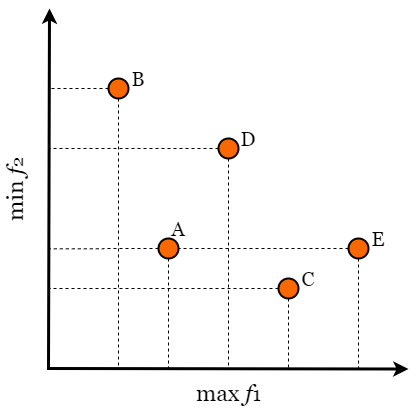
\includegraphics[scale=0.5]{images/pareto_dominance.png}
  \caption{
    Példa egy optimalizálási feladatra, ahol az $f_1$ célfüggvényt maximalizálni, míg az $f_2$ célfüggvényt minimalizálni kell.
  }
  \label{fig:PARETO_DOMINANCE}
\end{figure}


\subsection{Nash-dominancia}
A Nash-dominancia fogalmának bevezetése előtt szükséges néhány, a \textit{játékelméletből} \cite{von2007theory} ismert fogalom bevezetése.


\subsubsection{Nem-kooperatív játékok}
Legyen $n > 1$ természetes szám a játékosok száma, és $I = \left\{ 1, \dots, n \right\}$ a játékosok halmaza.
Minden $i \in I$ esetén, $S_i$ az $i$-edik játékos stratégiáinak a halmaza, míg $s_i \in S_i$ a játékos tetszőleges stratégiája.
Legyen $S = S_1 \times S_2 \times \dotsc \times S_n$ a stratégiaprofilok halmaza, $s \in S$ pedig egy általános stratégiaprofil.
Minden $i \in I$ esetén, $u_i \colon S \to \mathbb{R}$ az $i$-edik játékos kifizetőfüggvénye.
Legyen $U = \left\{ u_1, \dots, u_n \right\}$ a kifizetőfüggvények halmaza.
Jelölje $\left( t_i, s_{-i} \right)$ az $\left( s_1, \dots, s_{i-1}, t_i, s_{i+1}, \dots, s_n \right)$ stratégiaprofilt,
amelyet úgy kapunk, hogy az $s$ stratégiaprofil $i$-edik játékosának a stratégiáját kicseréljük $t_i$-re, $t_i \in S_i$.


\subsubsection{Nash-egyensúly}
Az előbb bevezetett jelölések segítségével bevezethetjük a nem-kooperatív játékelmélet központi fogalmát, a \textit{Nash-egyensúlyt} \cite{nash1951non}.

Azt mondjuk, hogy az $s^* \in S$ stratégiaprofil Nash-egyensúlyt alkot,
ha egyik játékosnak sem érdemes egyoldalúan eltérnie a stratégiaprofilban szereplő saját stratégiájától.
Tehát minden $i \in I$ játékos és $s_i \in S_i$ stratégia esetén, a következő egyenlőtlenség teljesül:
\[
  u_i\left(s^*\right) \ge u_i\left(t_i, s_{-i}^*\right).
\]


\subsubsection{Nash-dominancia}
A Nash-dominancia fogalmát \citeN{lung2008computing} vezették be, és a Nash-egyensúly fogalmán alapszik.

Legyen $x$ és $y$ két stratégiaprofil $S$-ből.
Bevezetünk egy $k \colon S \times S \to \mathbb{N}$ operátort, amely az $\left( x, y \right)$ pároshoz hozzárendeli a következő halmaz számosságát:
\[
  \left\{ i \in I \mid u_i(y_i, x_i) \ge u_i(x), y_i \neq x_i \right\}.
\]

A halmaz azon $i$ játékosokat tartalmazza, akik adott x stratégiaprofil esetén, hasznot húznának abból, ha megváltoztatnák stratégiájukat $x_i$-ről $y_i$-re.

Az $x$ stratégiaprofil akkor dominálja az $y$ stratégiaprofilt Nash értelemben ($x \prec y$), ha teljesül az alábbi feltétel:
\[
  k(x,y) < k(y, x).
\]

Tehát egy $x$ stratégiaprofil akkor dominál egy $y$ stratégiaprofilt, ha kevesebb játékos tudja megnövelni nyereségét úgy, hogy megváltoztatja stratégiáját $x_i$-ről $y_i$-re, mint fordítva.
Azt is mondhatjuk, hogy az $x$ stratégiaprofil stabilabb (közelebb van az egyensúlyhoz), mint az $y$ stratégiaprofil.


\subsubsection{Nash-optimum}
A Nash-dominancia segítségével bevezethetjük az optimum fogalmát.
Egy $s^* \in S$ stratégiaprofil Nash-optimum, ha nincs még egy olyan stratégiaprofil, ami dominálná őt:
\[
  \nexists s \in S, s \neq s^* \colon s \prec s^*.
\]


\subsubsection{Nash-front}
Gyakran megtörténik, hogy nem csak egy, hanem több Nash-optimális megoldásunk van.
Ebben az esetben a Nash-optimális megoldások halmazát nevezzük Nash-frontnak.


\subsubsection{Nash és a BOCNDP}
\citeN{lung2008computing} egy fontos következtetésre jutottak, miszerint minden Nash-egyensúlyt alkotó stratégiaprofil egyben Nash-optimum is, és minden Nash-optimum egyben Nash-egyensúlyt alkotó stratégiaprofil is.
Ez azért elengedhetetlenül fontos eredmény, mivel lehetővé teszi számunkra, hogy evolúciós kereső operátorok (keresztezés, mutáció, kiválasztás) segítségével megkeressük a Nash-egyensúlyt alkotó megoldásokat.


\subsection{Berge-dominancia}

